% Ivan Hip / 2019-05-08

\documentclass[croatian]{beamer}
\usetheme{Frankfurt}

% Ivan Hip / 2019-05-08
% iskustvo je pokazalo da kod korištenja Beamera treba učitati ove pakete

\usepackage[croatian]{babel}
\usepackage[utf8]{inputenc}
\usepackage[T1]{fontenc}
\usepackage{lmodern}

\hypersetup{unicode = true}

% Ivan Hip / 2019-05-08
% jedinstveni naslovni slajd za prezentacije

\newcommand{\naslov}[1]{
	\title{#1}
	\author{Ivan Hip}
	\institute{Geotehnički fakultet, Sveučilište u Zagrebu}
	\date{
\includegraphics[width=0.15\textwidth]{../CC-by-sa.pdf}}
} % \newcommand

\newcommand{\naslovnislajd}{
	\begin{frame}
		\titlepage
	\end{frame}
} % \newcommand

\naslov{Darcyjev zakon}

\begin{document}
\naslovnislajd

\section{Darcyjev zakon}
\begin{frame}{Darcyjev zakon}
\begin{itemize}
\item Darcyjev zakon opisuje tečenje kroz porozni medij, najčešće tlo 
\end{itemize}
\begin{block}{Uobičajeni zapis Darcyjevog zakona}
\[
v_{{\scriptscriptstyle _{D}}}=k\,i
\]
\begin{description}
\item [{$v_{{\scriptscriptstyle _{D}}}$}] -- Darcyjeva ili prividna brzina 
\item [{$k$}] -- koeficijent procjeđivanja (koeficijent filtracije) 
\item [{$i$}] -- hidraulički gradijent \smallskip{}
\end{description}
\end{block}
\begin{itemize}
\item razjasnit ćemo:
\begin{itemize}
\item zašto naziv prividna brzina? 
\item što je hidraulički gradijent? 
\item zašto je brzina proporcionalna hidrauličkom gradijentu? 
\end{itemize}
\end{itemize}
\end{frame}
%
\begin{frame}{Zašto naziv prividna brzina?}
\begin{itemize}
\item često se (i opravdano) umjesto $v_{{\scriptscriptstyle _{D}}}$ koristi
oznaka $q$ koja se interpretira kao protok po jediničnoj površini
presjeka 
\[
v_{{\scriptscriptstyle _{D}}}=q=\frac{Q}{S}
\]
\item ako je u eksperimentu izmjeren ukupni protok $Q$ kroz površinu presjeka
$S$ prividna (Darcyjeva) brzina $v_{{\scriptscriptstyle _{D}}}$
je ona brzina s kojom treba pomnožiti ukupnu površinu presjeka poroznog
materijala kroz koji je izmjeren protok $Q$ 
\item međutim, jasno je da protok nije moguć kroz ukupnu površinu presjeka,
jer se tekućina nalazi samo u porama poroznog materijala pa je stvarna
brzina tečenja uvjetovana udjelom pora u poroznom materijalu 
\end{itemize}
\end{frame}
%
\begin{frame}{Tekućina u porama poroznog materijala}
\begin{center}
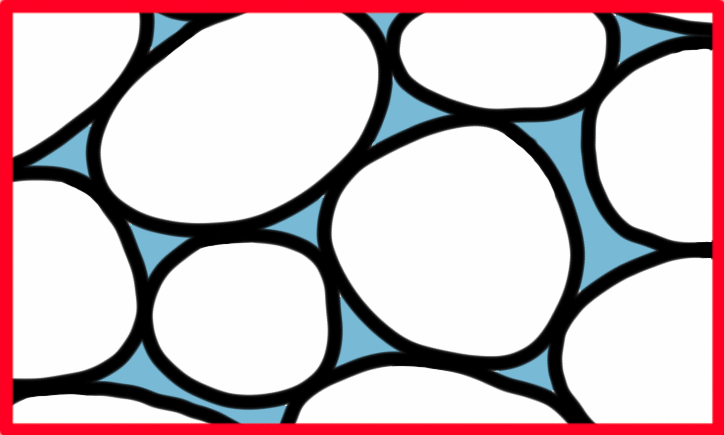
\includegraphics[height=0.55\paperheight]{slike/MF-11-tekucina-u-porama} 
\par\end{center}

\end{frame}
%
\begin{frame}{Poroznost}
\begin{itemize}
\item \emph{poroznost} je definirana kao omjer volumena pora i ukupnog volumena
\[
n\equiv\frac{V_{p}}{V}.
\]
\item kod tečenja je relevantna prvenstveno površina presjeka pa je \emph{efektivna
poroznost} $n_{\text{eff}}$ koja povezuje stvarnu, pravu srednju
brzinu $\bar{v}$ i prividnu brzinu $v_{{\scriptscriptstyle D}}$
\[
\bar{v}=\frac{v_{{\scriptscriptstyle _{D}}}}{n_{\text{ef}}}
\]
općenito manja od poroznosti $n$, to jest, općenito je $n_{\text{ef}}\leq n$ 
\end{itemize}
\begin{alertblock}{}
Kako je (efektivna) poroznost uvijek manja od jedan, jasno je da
je prava srednja brzina $\bar{v}$ uvijek veća od prividne Darcyjeve
brzine $v_{{\scriptscriptstyle _{D}}}$! 
\end{alertblock}
\end{frame}

\section{Hidraulički potencijal}
\begin{frame}{Hidraulički potencijal}
\begin{itemize}
\item da bi se moglo objasniti što je \emph{\alert{\emph{hidraulički gradijent}}}
prvo treba objasniti što je \emph{\alert{\emph{hidraulički potencijal}}} 
\item općenito, \emph{\alert{\emph{potencijal}}} je specifična potencijalna
energija u pojedinoj točki prostora (specifična u smislu: po jediničnom
naboju, po jediničnoj masi i sl.) 
\item pojam potencijala posebno važnu ulogu ima u elektrodinamici: napon
je razlika električnih potencijala, te zbog te razlike potencijala
(tj. napona) dolazi do tečenja električne struje 
\item analogija napona s hidrauličkim gradijentom: do tečenja tekućine dolazi
zbog razlike hidrauličkog potencijala, tj. hidrauličkog gradijenta 
\end{itemize}
\end{frame}
%
\begin{frame}{Gravitacijski potencijal u polju sile teže}
\begin{itemize}
\item gravitacijski potencijal je gravitacijska potencijalna energija tijela
jedinične mase u gravitacijskom polju 
\item potencijalna energija tijela mase $m$ u polju sile teže je 
\[
E_{p,G}=mgz
\]
\item gravitacijski potencijal u polju sile teže je potencijalna energija
tijela jedinične mase u polju sile teže 
\[
\varphi_{G}\equiv\frac{E_{p,G}}{m}=gz
\]
\item može se pokazati da je hidraulički potencijal u direktnoj vezi sa
specifičnom potencijalnom energijom tekućine u polju sile teže 
\end{itemize}
\end{frame}
%
\begin{frame}{Piezometarska visina je hidraulički potencijal}
\begin{itemize}
\item ukupna energijska visina je 
\[
H=\frac{p}{\rho g}+z+\frac{\bar{v}^{2}}{2g}
\]
\item suma prva dva člana, \emph{tlačne} i \emph{geodetske} visine, je \emph{piezometarska}
visina 
\[
h=\frac{p}{\rho g}+z
\]
zapravo potencijalna energija po jedinici težine tekućine 
\item gledano sa stanovišta fizike piezometarska visina je oblik potencijala
te se za $h$ koristi i naziv \emph{\alert{\emph{hidraulički potencijal}}} 
\item poput gravitacijskog potencijala i hidraulički potencijal je u najopćenitijem
obliku skalarna funkcija koordinata $x$, $y$ i $z$ 
\end{itemize}
\end{frame}

\section{Hidraulički gradijent}
\begin{frame}{Hidraulički gradijent između dvije točke}
\begin{alertblock}{}
\alert{Hidraulički gradijent} između dvije točke $A$ i $B$ definiran
je kao \textbf{razlika} piezometarskih visina u točkama $A$ i $B$
podijeljena s udaljenošću $L$ između točaka 
\[
i\equiv\frac{\Delta h}{L}=\frac{h_{_{A}}-h_{_{B}}}{L}
\]
\end{alertblock}
\begin{itemize}
\item ako je specifična potencijalna energija tekućine u točkama $A$ i
$B$ jednaka (tj. $i=0$) nema razloga da bi tekućina tekla iz $A$
u $B$, ili iz $B$ u $A$ 
\item tek kada postoji razlika hidrauličkih potencijala, tekućina teče s
mjesta gdje ima veći potencijal prema mjestu gdje ima manji, tj. \alert{tekućina teče u smjeru smanjenja specifične potencijalne energije!} 
\end{itemize}
\end{frame}
%
\begin{frame}{Hidraulički gradijent kod otvorenog toka}
\begin{alertblock}{}
\alert{Kod jednolikog tečenja} u otvorenim koritima ne mijenja
se dubina toka, tj. $y_{_{A}}=y_{_{B}}$ pa slijedi 
\[
i=\frac{h_{_{A}}-h_{_{B}}}{L}=\frac{y_{_{A}}+z_{_{A}}-(y_{_{B}}+z_{_{B}})}{L}=\frac{z_{_{A}}-z_{_{B}}}{L}=I
\]

dakle, \alert{hidraulički gradijent jednak je nagibu dna!} 
\end{alertblock}
\begin{itemize}
\item srednja brzina tečenja u otvorenim koritima proporcionalna je korijenu
iz nagiba dna, tj. hidrauličkog gradijenta 
\[
\bar{v}\propto\sqrt{I}=\sqrt{i}
\]
\item međutim, hidraulički gradijent može se definirati i u svakoj pojedinoj
točki prostora 
\end{itemize}
\end{frame}
%
\begin{frame}{Hidraulički gradijent u točki (1D primjer)}
\begin{itemize}
\item najjednostavnije je promatrati jednodimenzionalan slučaj kad je hidraulički
potencijal $h$ funkcija samo jedne koordinate $x$ 
\item udaljenost između točaka $A$ i $B$ je 
\[
L=x_{_{B}}-x_{_{A}}
\]
\item točka $B$ može se proizvoljno približavati točki $A,$ to jest udaljenost
$L$ smanjivati prema nuli ($L\rightarrow0$) pa je hidraulički gradijent
u točki $A$ definiran kao 
\[
i(x_{_{A}})\equiv-\lim_{L\rightarrow0}\frac{h(x_{_{A}}+L)-h(x_{_{A}})}{L}=\left.-\frac{dh(x)}{dx}\right|_{x=x_{A}}
\]
\item negativan predznak uvodi se jer je tečenje uvijek s višeg prema nižem
potencijalu! 
\end{itemize}
\end{frame}
%
\begin{frame}{Hidraulički gradijent je gradijent hidrauličkog potencijala}
\begin{block}{}
U dvije ili tri dimenzije hidraulički potencijal je funkcija dvije
$h(x,\,y)$ ili tri $h(x,\,y,\,z)$ koordinate, a hidraulički gradijent
je vektor 
\[
\vec{I}\equiv-\vec{\nabla}h
\]
\end{block}
\begin{alertblock}{Vektorski zapis Darcyjevog zakona u tri dimenzije}
\[
\vec{v}_{_{D}}=k\,\vec{I}=-k\,\vec{\nabla}h(x,\,y,\,z)
\]
\end{alertblock}
Za homogeno tlo $k=konst.$, ali ako je tlo nehomogeno $k$ može biti
različit u svakoj točki pa je $k$ zapravo skalarna funkcija koordinata
i 
\[
\vec{v}_{_{D}}=-k(x,\,y,\,z)\vec{\nabla}h(x,\,y,\,z)
\]
\end{frame}
%
\begin{frame}{Koeficijent procjeđivanja}
\begin{itemize}
\item u najopćenitijem slučaju tlo može biti nehomogeno i anizotropno pa
$k$ postaje simetrični tenzor 
\[
k=\left[\begin{array}{ccc}
k_{xx} & k_{xy} & k_{xz}\\
k_{yx} & k_{yy} & k_{yz}\\
k_{zx} & k_{zy} & k_{zz}
\end{array}\right]
\]
\item ipak, u praksi je vrlo teško odrediti $k$ u svakoj točki tla, tako
da se uglavnom aproksimira s jednom skalarnom vrijednošću koja je
tipična za pojedinu vrstu tla 
\item koeficijent procjeđivanja mjeri se u metrima u sekundi, a u literaturi
se često koristi i naziv \emph{koeficijent filtracije} 
\end{itemize}
\end{frame}
%
\begin{frame}{Tipične vrijednosti koeficijenta procjeđivanja vode}
\begin{center}
\begin{tabular}{|l|c|}
\hline 
\emph{Vrsta tla}  & $k$ {[}m/s{]}\tabularnewline
\hline 
\hline 
čisti šljunak  & $10^{-2}$ i veće\tabularnewline
\hline 
čisti pijesak  & $10^{-2}$ do $10^{-4}$\tabularnewline
\hline 
pijesak granulirani  & $10^{-4}$ do $5\cdot10^{-5}$\tabularnewline
\hline 
sitni pijesak  & $5\cdot10^{-4}$ do $10^{-5}$\tabularnewline
\hline 
prašinasti do zamuljeni pijesak  & $2\cdot10^{-5}$ do $10^{-6}$\tabularnewline
\hline 
prašina i mulj  & $5\cdot10^{-6}$ do $10^{-7}$\tabularnewline
\hline 
glina  & $10^{-7}$ i manje \tabularnewline
\hline 
\end{tabular}
\par\end{center}
\vfill{}
 Izvor: \emph{Jović, V.: ``Osnove hidromehanike'', Element, Zagreb
2006.} 
\end{frame}

\section{Granice valjanosti Darcyjevog zakona}
\begin{frame}{Usporedba s tečenjem u otvorenim koritima}
\begin{block}{}
Kod usporedbe Darcyjevog zakona s tečenjem u otvorenim koritima upada
u oči jedna na prvi pogled neobična i neočekivana razlika:
\begin{itemize}
\item brzina tečenja je u Darcyjevom zakonu proporcionalna hidrauličkom
gradijentu 
\[
\bar{v}\propto i
\]
\item brzina tečenja kod tečenja u otvorenim koritima proporcionalna \alert{korijenu}
iz nagiba dna, tj. hidrauličkog gradijenta 
\[
\bar{v}\propto\sqrt{I}=\sqrt{i}
\]
\end{itemize}
\end{block}
Sjetimo se: faktor $\sqrt{I}$ pojavljuje se i u Chezyjevoj i u Manningovoj
formuli, a direktno slijedi i iz Darcy-Weisbachove formule 
\[
h_{f}=\lambda\frac{L}{D}\frac{\bar{v}^{2}}{2g}\quad\Rightarrow\quad I=\frac{h_{f}}{L}=\frac{\lambda}{D}\frac{\bar{v}^{2}}{2g}\quad\Rightarrow\quad\bar{v}=\sqrt{\frac{2gD}{\lambda}}\sqrt{I}
\]

\end{frame}
%
\begin{frame}{Za porozni medij tipično je laminarno tečenje}

Po čemu se tečenje u otvorenim koritima razlikuje od tečenja u poroznim
materijalima? 
\begin{itemize}
\item korita su mnogo puta veća od pora kroz koje teče voda u tlu! 
\item brzina tečenja u otvorenim koritima obično mnogo veća od brzine tečenja
vode u tlu 
\item upravo su karakteristična dimenzija sustava $D$ i srednja brzina
tečenja $\bar{v}$ ključni faktori kod izračunavanja Reynoldsovog
broja 
\[
\text{Re}\equiv\frac{\bar{v}\,D}{\nu}
\]
\item za tečenje u otvorenim koritima tipične su velike vrijednosti Reynoldsovog
broja $\Rightarrow$ gotovo uvijek turbulentni režim tečenja 
\item međutim, male dimenzije pora i male brzine tečenja u tlu dovode do
malih vrijednosti Reynoldsovog broja $\Rightarrow$ za porozni medij
tipično laminarno tečenje 
\end{itemize}
\end{frame}
%
\begin{frame}{Laminarno tečenje proporcionalno hidrauličkom gradijentu}
\begin{itemize}
\item uvrštavanjem poznatog koeficijenta otpora kod laminarnog tečenja $\lambda=\frac{64}{Re}$
u Darcy-Weisbachovu formulu slijedi 
\[
h_{f}=\frac{64}{\text{Re}}\frac{L}{D}\frac{\bar{v}^{2}}{2g}=\frac{64\nu}{\bar{v}D}\frac{L}{D}\frac{\bar{v}^{2}}{2g}=\frac{32\nu}{g}\frac{L}{D^{2}}\bar{v}
\]
iz čega možemo izraziti srednju brzinu kao funkciju hidraličkog gradijenta
\[
\bar{v}=\frac{g\,D^{2}}{32\nu}\,\frac{h_{f}}{L}=\frac{g\,D^{2}}{32\nu}\,I
\]
\end{itemize}
\begin{alertblock}{}
Za laminarno tečenje tipično je da je srednja brzina tečenja proporcionalna
hidrauličkom gradijentu, tj. tipična je linearna ovisnost $\bar{v}\propto I$,
kao što je to slučaj u Darcyjevom zakonu! 
\end{alertblock}
\end{frame}
%
\begin{frame}{Gornja granica valjanosti Darcyjevog zakona}
\begin{alertblock}{}
Darcyjev zakon zapravo nije temeljni fizikalni zakon, već je manifestacija
(posljedica) laminarnog režima tečenja tipičnog za materijale s malim
dimenzijama pora. 
\end{alertblock}
\begin{block}{}
Očigledno je ograničenje na valjanost i primjenu Darcyjevog zakona:
kod većih dimenzija pora i sve veće brzine tečenje, tečenje prelazi
iz laminarnog u turbulentno i Darcyjev zakon više ne vrijedi! 

\end{block}
Općenito možemo pisati
\[
\bar{v}=k\,I^{\alpha}
\]

\begin{itemize}
\item za male vrijednosti Reynoldsovog broja $\alpha=1$ (Darcyjev zakon) 
\item s porastom Reynoldsovog broja $\alpha$ se postepeno mijenja te za
velike vrijednosti postaje $\frac{1}{2}$ ($\bar{v}\propto\sqrt{I}$)
--- što je tipično za sustave koji su duboko u turbulentnom režimu
tečenja. 
\end{itemize}
\end{frame}
%
\begin{frame}{Donja granica valjanosti Darcyjevog zakona}
\begin{itemize}
\item postoji i donja granica valjanosti Darcyjevog zakona: kod nekih materijala
tečenja uopće neće biti dok hidraulički gradijent ne dosegne neku
kritičnu vrijednost 
\item primjer takvih materijala, odnosno vrste tla, su gline\vfill{}
 \vfill{}
 \vfill{}
 \vfill{}
 \vfill{}
 \vfill{}
 \vfill{}
 
\end{itemize}
\end{frame}
%
\begin{frame}{Literatura}
\begin{itemize}
\item Jović, V.: \emph{``Osnove hidromehanike''}, Element, Zagreb 2006.
(9.~poglavlje: \emph{``Strujanje podzemnih voda''}) 
\item Miletić, P., Heinrich Miletić M.: \emph{``Uvod u kvantitativnu hidrogeologiju''},
Varaždin 1981. (2. poglavlje: \emph{``Voda u podzemlju''})\vfill{}
 \vfill{}
 \vfill{}
 \vfill{}
 \vfill{}
 
\end{itemize}
\end{frame}

\end{document}
